%	MODULO PER LA COMUNICAZIONE
% socket
% passaggio ip
% protocollo comunicazione

La comunicazione fra i robot � stata implementata tramite socket tcp. Tale tecnologia ha permesso, avendo conoscenza degli indirizzi IP di tutti i robot partecipanti, di costruire delle linee di comunicazione punto-punto. Come gi� visto nella sezione introduttiva, il gioco prevede due ruoli: solo i robot ricoprenti ruoli diversi si scambiano messaggi.

\subsection{Gestione delle Socket}

Ogni robot gestisce almeno una socket: il Role Manager del nodo Witch ne gestisce una per ogni robot Kid e i Role Manager dei nodi Kid ne gestiscono una soltanto. Le socket, a prescindere dalla tipologia di nodo, vengono gestite attraverso il metodo \texttt{manageSocket} della classe \texttt{RoleManager}. Il metodo in questione prende in input il file descriptor della socket su cui si metter� in ascolto e a cui invier� messaggi. \texttt{manageSocket} viene eseguito da un thread a parte, generato nel metodo \texttt{createAndStartConnection} con l'unico compito di gestirla. In particolare, abbiamo che i nodi Kid generano un solo nuovo thread e il nodo Witch genera un thread per ogni nodo Kid a cui deve connettersi. Tale metodo non fa altro che rimanere in ascolto della socket passatagli finch� la variabile d'istanza \texttt{stopThread} assume valore \texttt{true}: ci� accade quando la partita in corso � terminata e bisogna resettare i parametri della classe \texttt{RoleManager}. I messaggi che arrivano sulla socket vengono quindi intercettati all'interno di questo loop e gestiti da un array di \textit{handlers} il quale, a seconda del tipo di messaggio ricevuto, invoca il metodo responsabile della gestione di quest'ultimo. Una volta usciti dal "loop di ascolto" il thread in questione viene fermato. 

ROS permette la definizione di variabili globali al sistema, referenziabili a run-time dai diversi nodi. Si � scelto di sfruttare questa possibilit� offerta da ROS per comunicare ai robot gli indirizzi IP di tutti i partecipanti, incluso il proprio. I primi memorizzati in una lista di stringhe e il secondo in una semplice stringa, queste variabili vengono impostate una volta sola (dopo aver eseguito \textit{roscore}) attraverso le due istruzioni seguenti e recuperate nel metodo \texttt{\_\_init\_\_} del nodo \texttt{RoleManager}.
\begin{center}
	\texttt{setparam /ipList "['100.101.0.10', '100.101.0.11', '100.101.0.12']"}
	\texttt{setparam /myIPAddress "100.101.0.10"}
\end{center}

\subsection{Il Protocollo di Comunicazione}

	Il protocollo di comunicazione � molto semplice: la struttura statica del gioco ha permesso la definizione di un protocollo rigido. I messaggi vengono scambiati solo tra giocatori di ruoli diversi, in particolare tra i Kids e la Witch: questo spiega la scelta di collegamenti punto-punto delle socket.
	Sono stati previsti tre tipi di messaggio:
	\begin{itemize}
		\item un messaggio in cui la Witch comunica a tutti i Kids il colore da toccare, dando cos� il via al gioco;
		\item un messaggio in cui un Kid comunica alla Witch di aver appena toccato il colore comunicatogli;
		\item un messaggio in cui la Witch comunica a tutti i Kids che il gioco � terminato e chi fra loro � il perdente.
	\end{itemize}
	Una descrizione grafica del protocollo di comunicazione � presentata in Figura~\ref{fig:communicationprotocol}.
	
	% Figura protocollo di comunicazione
	\begin{figure}
		\centering
		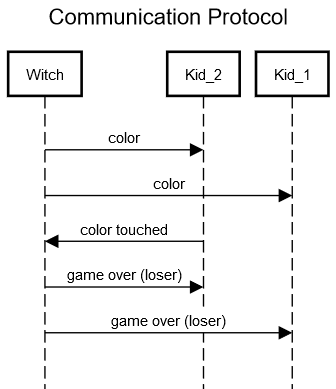
\includegraphics[width=0.7\textwidth]{images/CommunicationProtocol.png}
		\caption{Rappresentazione grafica del protocollo di comunicazione.}
		\label{fig:communicationprotocol}
	\end{figure}